% ======================================================================
\documentclass[12pt,a4paper,twoside,openright]{book}

%───────── Auxiliary packages ──────────────────────────────────────────
\usepackage{blindtext}
\usepackage{mwe}
\usepackage{csquotes}
\usepackage{graphicx}
\usepackage{booktabs}
\usepackage{tabularx}
\usepackage{siunitx}
\usepackage{amsmath,amssymb}
\usepackage{algorithm}
\usepackage{algpseudocode}
\usepackage{listings}
\usepackage{nomencl}
\makenomenclature
\usepackage[
  backend=biber,
  style=numeric,
  sorting=nyt
]{biblatex}
\usepackage{subcaption}
\setlength{\textfloatsep}{20pt} % Separación entre el fin de una imagen y el parrafo siguiente (sin esto, el hueco era demasiado grande)
\captionsetup[subfigure]{skip=2pt}
\addbibresource{references.bib}


% Listings config
\lstset{
  basicstyle=\ttfamily\small,
  numbers=left,
  numberstyle=\tiny,
  columns=fullflexible,
  frame=single,
  breaklines=true,
  tabsize=2
}

%───────── Template, covers, back cover ────────────────────────────────
\usepackage{template/sty_files/template-TFGspanish-uma}

\usepackage{template/sty_files/cotutor_cover-blueuma}
\usepackage{template/sty_files/cotutor_cover-whiteuma}

\usepackage{template/sty_files/backcover-uma}
\usepackage{parskip}

%======================================================================
\begin{document}

%────────────────────── Blue front cover (Cotutor) ───────────────────────

\MakeBlueUMACover{
  degree     = {Grado en Ingeniería Informática},
  mencion    = {Mención en Computación},
  titleES    = {Diseño e implementación de un agente de razonamiento basado en LLMs con exploración mediante Beam Search},
  titleEN    = {Design and implementation of an LLM-based reasoning agent with Beam Search exploration},
  author     = {Juan Torres Gómez},
  tutor      = {Sergio Gálvez Rojas},
  % cotutor= {Dra.~Jane Doe},
  dept       = {Departamento de Lenguajes y Ciencias de la Computación},
  cityDate   = {Málaga, Julio, 2026},
  logoLeft   = {template/logos/NEG-uma-logo.png},
  logoRight  = {template/logos/NEG-etsi-logo.png}
}

%────────────────────── White front cover (Cotutor) ───────────────────────
\MakeWhiteUMACover{
  degree     = {Grado en Ingeniería Informática},
  mencion    = {Mención en Computación},
  titleES    = {Diseño e implementación de un agente de razonamiento basado en LLMs con exploración mediante Beam Search},
  titleEN    = {Design and implementation of an LLM-based reasoning agent with Beam Search exploration},
  author     = {Juan Torres Gómez},
  tutor      = {Sergio Gálvez Rojas},
  % cotutor= {Dra.~Jane Doe},
  dept       = {Departamento de Lenguajes y Ciencias de la Computación},
  cityDate   = {Málaga, Julio, 2026},
  defenseDate = {Julio, 2026},
  logoLeft   = {template/logos/POS-uma-logo.png},
  logoRight  = {template/logos/POS-etsi-logo.png}
}

\frontmatter

%────────────────────── Abstracts ──────────────────────────────────────
\renewcommand{\abstractname}{Resumen}
\begin{abstract}
\setlength{\parindent}{0pt}
\setlength{\parskip}{0.6em}

En este trabajo se presenta el desarrollo de una prueba de concepto de un agente con capacidad de razonamiento basado en modelos de lenguaje de gran tamaño \emph{(LLMs)}.
A diferencia de los sistemas tradicionales que generan una respuesta directa ante una consulta, el agente propuesto implementa bucles dinámicos de \emph{Chain of Thought (CoT)} que le permiten generar,
evaluar y refinar pasos intermedios antes de producir una respuesta final.

El sistema se implementa utilizando modelos de lenguaje ejecutados en local, como Llama-3, junto con la librería \emph{LangGraph} para la contrucción de flujos de razonamiento. Además, se emplea
una estrategia de búsqueda basada en \emph{Beam Search} que permite explorar múltiples posibles líneas de razonamiento y seleccionar aquellas más prometedoras mediante un mecanismo de puntuación.

El objetivo del proyecto es analizar la viabilidad de este enfoque para mejorar la capacidad de razonamiento de agentes basados en LLMs y estudiar su comportamiento en diferentes escenarios de
resolución de problemas.
\medskip

\noindent \textbf{Palabras clave:} modelos de lenguaje, agentes inteligentes, \emph{Chain of Thought}, razonamiento automático, \emph{Beam Search}.
\end{abstract}


\renewcommand{\abstractname}{Abstract}
\begin{abstract}
\setlength{\parindent}{0pt}
\setlength{\parskip}{0.6em}

This work represents the development of a proof-of-concept reasoning agent based on Large Language Models \emph{(LLMs)}.
Unlike traditional systems that generate an immediate response to a query, the proposed agent implements dynamic \emph{Chain Of Thought (CoT)} loops that allow it to generate, evaluate, and refine
intermediate reasoning steps before producing a final answer.

The system is implemented using locally executed language models such as Llama-3, together with the \emph{LangGraph} library for building reasoning workflows. Additionally, a \emph{Beam Search}
strategy is employed to explore multiple possible reasoning paths and select the most promising ones through a scoring mechanism.

The goal of this project is to analyze the feasibility of this approach to improve the reasoning capabilities of LLM-based agents and to study their behaviour in different problem-solving scenarios.
\medskip

\noindent \textbf{Keywords:} language models, intelligent agents, \emph{Chain of Thought}, automated reasoning, \emph{Beam Search}.
\end{abstract}

%──────────────── Acknowledgments ───────────────────────────────────────

% ====================================== AGRADECIMIENTOS ====================================
\begin{umaacknowledgments}
Agradezco su función a los clínicos colaboradores, así como al grupo de Inteligencia Computacional y Análisis de Imagen de la Universidad de Málaga.
\end{umaacknowledgments}

%────────────────────── TOC and lists ──────────────────────────────────
\clearpage
\tableofcontents
\clearpage
\listoffigures
\clearpage
\listoftables
\clearpage

%────────────────────── Nomenclature ───────────────────────────────────
\nomenclature{$x \in \mathbb{R}^{H\times W\times D}$}{HR volume}
\nomenclature{$y \in \mathbb{R}^{h\times w\times d}$}{LR volume}
\nomenclature{$A$}{Forward operator (blur+downsample)}
\nomenclature{$\hat x$}{Network reconstruction}
\nomenclature{$\mathcal{L}$}{Training objective}
\nomenclature{$\operatorname{PSNR}$}{Peak Signal-to-Noise Ratio}
\nomenclature{$\operatorname{SSIM}$}{Structural Similarity}
\nomenclature{$\operatorname{Dice}$}{Sørensen–Dice coefficient}
\printnomenclature
\clearpage

\mainmatter
%────────────────────── Capítulo 1 — Introducción ───────────────────────
\chapter{Introducción}
\section{Motivación}
%\setlength{\parindent}{0pt}
%\setlength{\parskip}{0.5em}

En los últimos años, el desarrollo de los \emph{Large Language Models (LLMs)} ha supuesto un avance significativo en tareas de procesamiento
del lenguaje natural. Sin embargo, a pesar de la capacidad para generar texto coherente y resolver una amplia variedad de tareas, estos modelos
presentan limitaciones en lo que a enfrentar problemas que requieren un razonamiento complejo se refiere, ya que tienden a generar respuestas
directas sin una estructura intermedia explícita.

La ausencia de pasos intermedios limita la capacidad de valorar el razonamiento, desencadenando en falta de transparencia y control sobre cómo se
construye el razonamiento.
Es por ello que surge la necesidad de desarrollar sistemas que no solo generen respuestas, sino que estructuren su proceso de razonamiento y evalúen
sus propios pasos intermedios, con un enfoque que facilite la experimentación y análisis del comportamiento del modelo.

En conclusión, este proyecto se plantea a partir de la motivación por construir algo más complejo que una simple llamada a un modelo, profundizando
así en un área en crecimiento, desde el interés por entender no solo qué responden estos modelos, sino cómo llegan a hacerlo.

\section{Trabajos previos}

Con el fin de abordar la limitación que presentan los \emph{Large Language Models (LLMs)} anteriormente mencionada, diversos trabajos han propuesto
técnicas que fomentan el razonamiento paso a paso. Un ejemplo de esto es \emph{"Chain-of-Though Prompting (CoT)"}, introducido por Wei et al. (2022) [1],
el cual consiste en guiar al modelo para que genere pasos intermedios antes de alcanzar una respuesta final. Este enfoque pone de manifiesto la importancia
de estructurar el proceso de generación en lugar de limitarse a obtener una respuesta final directa.

Por otro lado, en el ámbito de la generación de texto, los algoritmos de búsqueda han sido ampliamente utilizados para explorar múltiples
posibles soluciones. Destaca el algoritmo de \emph{Beam Search}, el cual se apoya en una función de evaluación para mantener las secuencias más
prometedoras en cada iteración. Trabajos como el de Wu et al. (2020) [3] demuestran que, aunque este método haya sido tradicionalmente aplicado en tareas como la traducción automática,
su uso puede extenderse también al razonamiento en \emph{LLMs}, simplemente permitiendo explorar distintas cadenas de pensamiento
\emph{(CoT)} y seleccionando las más relevantes (según la función de evaluación anteriormente mencionada).

Estos antecedentes reflejan dos ideas fundamentales:
\begin{itemize}
  \item Por un lado, la necesidad de guiar el razonamiento de los modelos mediante la generación de pasos intermedios.
  \item Por el otro, la utilidad de explorar múltiples soluciones antes de seleccionar la respuesta final.
\end{itemize}

Sin embargo, la combinación de ambos enfoques en sistemas que implementen bucles dinámicos de razonamiento y mecanismos de selección de hipótesis
continua siendo un área en pleno desarrollo.

\section{Objetivos}

El objetivo principal de este trabajo es desarrollar una prueba de concepto de un agente basado en modelos de lenguaje capaz de incorporar un proceso de
razonamiento estructurado, en lugar de generar respuestas de forma directa. De esta forma, y con el objetivo de facilitar un aálisis detallado del proceso
seguido por el modelo, se busca explorar un enfoque que permita descomponer la resolución de un problema de índole lingüística en una serie de pasos intermedios.

De forma más concreta, se pretende implementar un sistema que no dependa únicamente de un camino de razonamiento, sino que sea capaz de generar múltiples posibles
trayectorias, permitiendo así analizar y estudiar como evoluciona el proceso de generación de cada una de ellas. Asimismo, un mecanismo evaluará la calidad de dichos
razonamientos generados, con el fin de seleccionar aquellos que resulten más adecuados con el tipo de problema que con el que se está trabajando. Este proceso de
evaluación se utilizará por tanto para guiar la exploración del espacio de soluciones, descartando las opciones menos prometedoras.

Otro gran objetivo de este proyecto se centra en la estructuración del funcionamiento del sistema mediante un flujo de ejecución organizado, que facilite no solo la
comprensión de este, sino también su posible extensión en trabajos futuros.

Por último, se busca analizar el comportamiento del agente desarrollado a través de problemas de índole lingüística...


\section{Estructura del proyecto}

%────────────────────── Chapter 2 — Fundamentals ───────────────────────
\chapter{Fundamentals}
\section{Imaging model and objectives}
Assume \(y = A x + n\). The SR network \(f_\theta\) estimates
\(\hat x = f_\theta(y)\).
We use the composite objective
\begin{equation}
  \mathcal{L}_{\mathrm{SR}}
  = \lambda_1 \lVert \hat x - x \rVert_1
  + \lambda_s \left(1-\operatorname{SSIM}(\hat x, x)\right)
  + \lambda_{\mathrm{tv}} \operatorname{TV}(\hat x).
  \label{eq:sr_loss}
\end{equation}
For segmentation logits \(z = g_\phi(\hat x)\) and mask \(m\),
\begin{equation}
  \mathcal{L}_{\mathrm{seg}}
  = 1 - \operatorname{Dice}\!\left(\sigma(z), m\right)
    + \beta\, \operatorname{CE}\!\left(\sigma(z), m\right).
  \label{eq:seg_loss}
\end{equation}
Total loss:
\(\mathcal{L} = \mathcal{L}_{\mathrm{SR}} + \gamma\,\mathcal{L}_{\mathrm{seg}}\).

\section{Metrics}
Performance metrics
\begin{align}
\operatorname{PSNR}(x,\hat x) &= 10\log_{10}\!\frac{L^2}{\operatorname{MSE}(x,\hat x)},\\
\operatorname{SSIM}(x,\hat x) &= \frac{(2\mu_x\mu_{\hat x}+C_1)(2\sigma_{x\hat x}+C_2)}
{(\mu_x^2+\mu_{\hat x}^2+C_1)(\sigma_x^2+\sigma_{\hat x}^2+C_2)},\\
\operatorname{Dice}(p,m) &= \frac{2\sum p m}{\sum p + \sum m}.
\end{align}

%────────────────────── Chapter 3 — LangGraph ────────────────────────────
\chapter{LangGraph}
\section{Introducción a LangGraph}

En los sistemas basados en modelos de lenguaje, el enfoque tradicional ha consistido en realizar llamadas independientes y aisladas a un modelo, evolucionando posteriormente
hacia sistemas más complejos capaces de gestionar flujos de ejecución estructurados. Esto cambio responde así a la necesidad de construir aplicaciones que no solo generen
respuestas, sino que integren múltiples pasos de procesamiento, toma de decisiones y manejo de información intermedia.

En este contexto surge \emph{LangGraph}, una herramienta que se presenta como alternativa a los enfoques lineales, y diseñada para facilitar la construcción de agentes
mediante la definición de flujos de ejecución basados en grafos. \emph{LangGraph} modela procesos de forma más flexible, en los que pueden existir bifurcaciones, ciclos y
dependencias entre distintos pasos. \cite{langgraph2024}

A diferencia de un flujo secuencial, un grafo permite mayor flexibilidad, al representar de manera más natural procesos complejos, en los que el sistema puede iterar,
tomar decisiones en función del estado actual o repetir determinadas operaciones hasta alcanzar un resultado adecuado. Este tipo de estructura es clave en sistemas que requieren
un comportamiento dinámico, como es el caso de agentes con capacidad de razonamiento iterativo.

\begin{figure}[h]
    \centering

    \begin{subfigure}{0.45\textwidth}
        \centering
        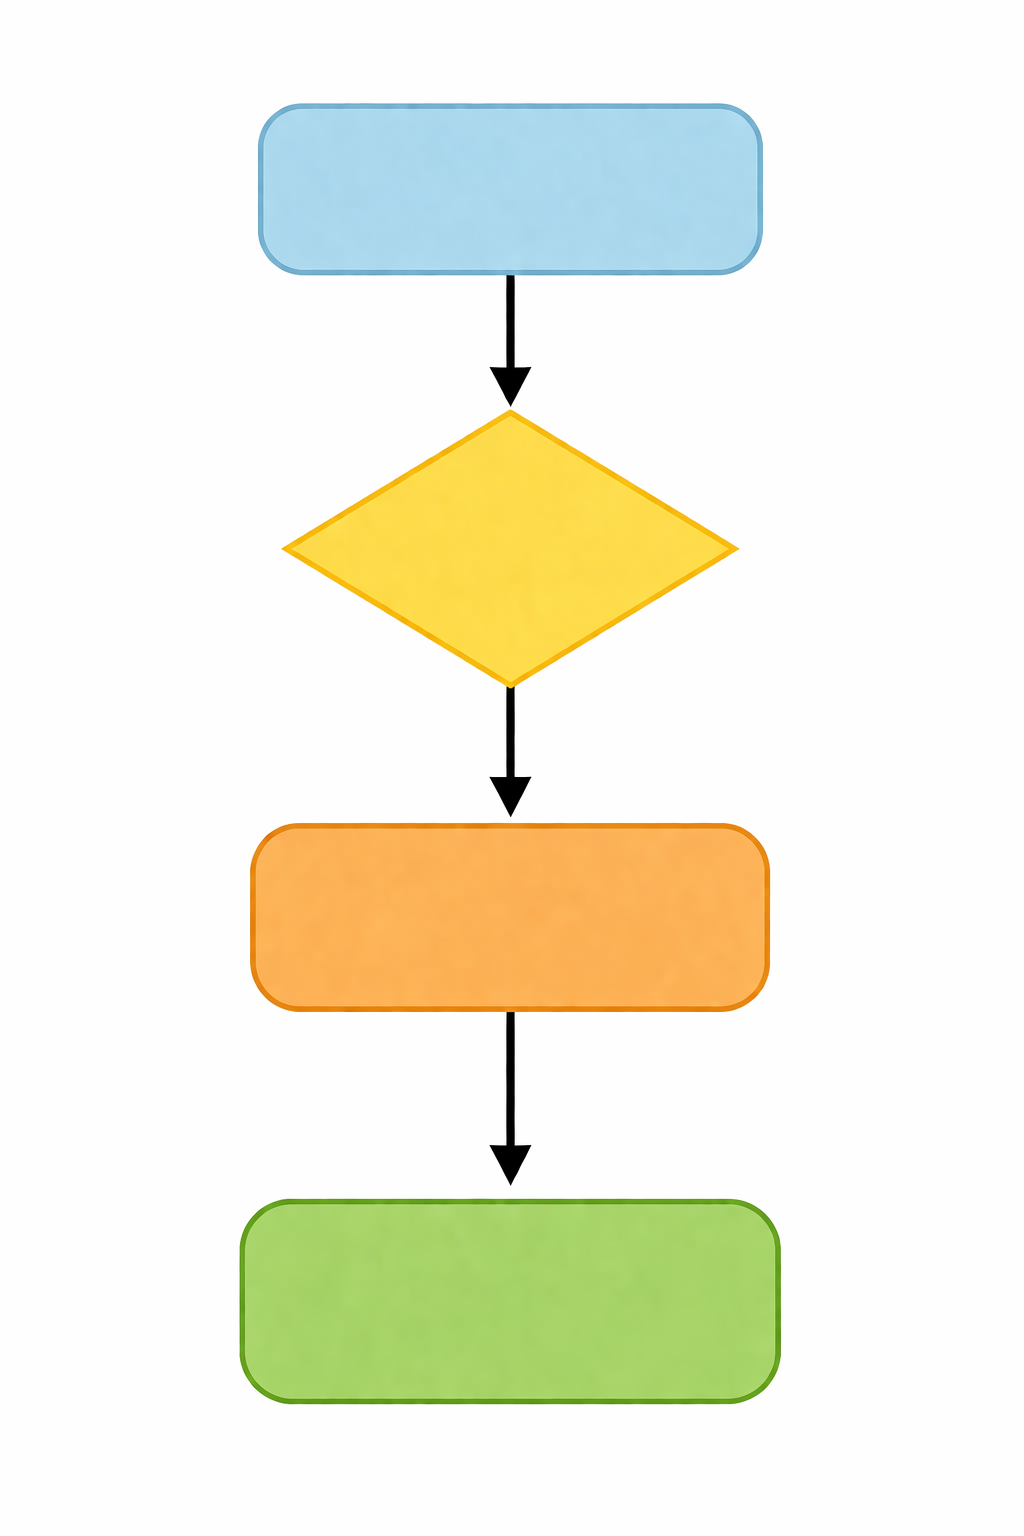
\includegraphics[width=0.8\linewidth]{images/DiagramaFlujoSecuencial.png}
        \caption{Ejemplo de enfoque tradicional mediante diagrama de flujo lineal}
    \end{subfigure}
    \hfill
    \begin{subfigure}{0.45\textwidth}
        \centering
        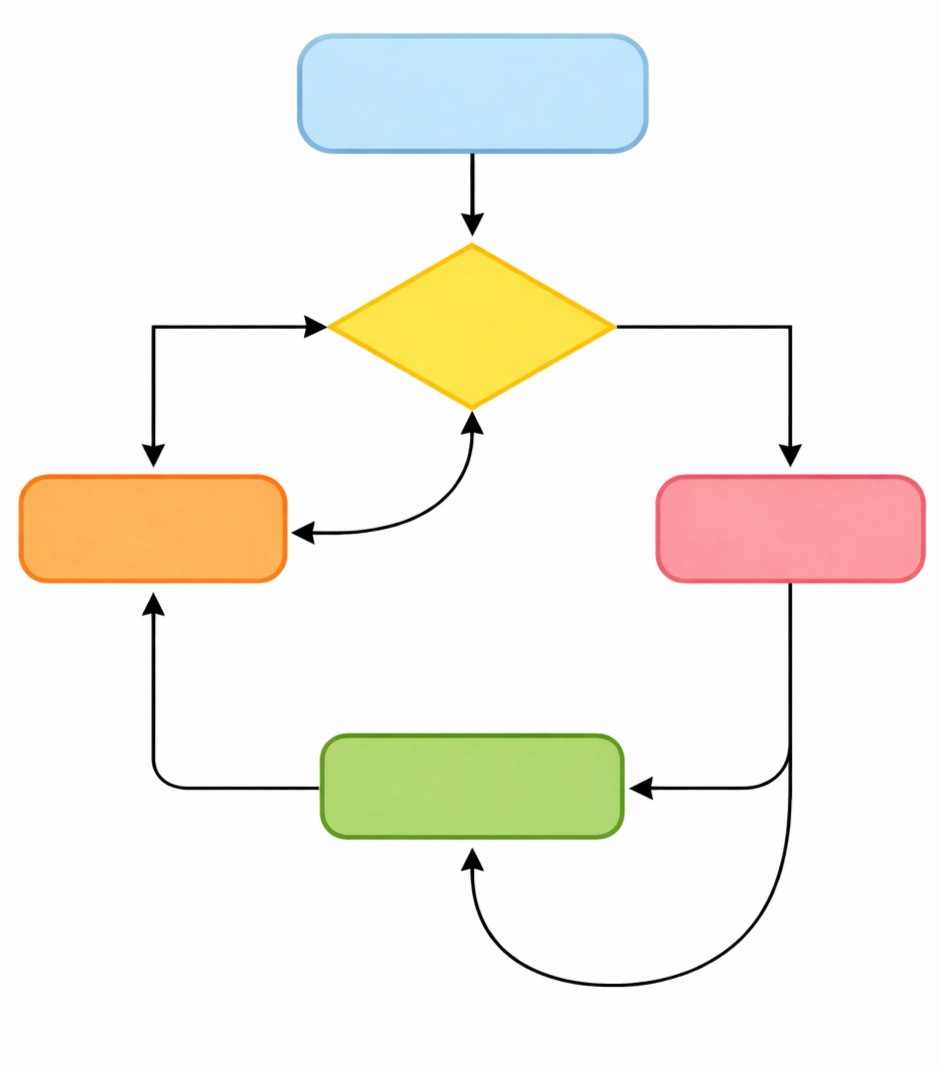
\includegraphics[width=\linewidth]{images/DiagramaFlujoGrafo2.png}
        \caption{Ejemplo de enfoque moderno mediante diagrama de flujo en grafo}
    \end{subfigure}

    \caption{Comparación entre enfoques. Fuente: Elaboración propia}
\end{figure}

Además, la modularidad que ofrece \emph{LangGraph} al facilitar la separación de responsabilidades dentro del sistema, permitiendo definir distintos componentes que se encargan de
tareas específicas no solo mejorar la claridad del diseño, sino que a su vez favorece la reutilización y extensión del sistema. Algunas de las tareas específicas ejecutadas por los
compenentes son la generación de contenido, la evaluación de resultados o la actualización del estado interno.

De este modo, \emph{LangGraph} constituye una base sólida para el desarrollo de agentes avanzados, proporcionando un marco de trabajo que permite superar las limitaciones de los
enfoques secuenciales tradicionales y ofreciendo una forma más estructurada y flexible de diseñar agentes basados en modelos de lenguaje.

%\begin{algorithm}
%\caption{Joint SR+Seg training}
%\label{alg:train}
%\begin{algorithmic}[1]
%\Procedure{Train}{$\mathcal{D}$, $\theta$, $\phi$}
%  \For{epoch $=1..E$}
%    \For{batch $(y,x,m)\sim \mathcal{D}$}
%      \State $\hat x \gets f_\theta(y)$
%      \State $z \gets g_\phi(\hat x)$; $p\gets\sigma(z)$
%      \State $\mathcal{L}\gets \mathcal{L}_{\mathrm{SR}}(\hat x,x)+\gamma\,\mathcal{L}_{\mathrm{seg}}(p,m)$
%      \State Update $(\theta,\phi)$ by Adam on $\nabla \mathcal{L}$
%    \EndFor
%  \EndFor
%\EndProcedure
%\end{algorithmic}
%\end{algorithm}

%────────────────────── Mathematical Foundations ──────────────────────────
\section{Mathematical foundations}

\begin{definition}[label=def:ssim]{Structural Similarity Index}
The \textbf{Structural Similarity Index (SSIM)} between two images $x$ and $\hat{x}$ is defined as:
\[
\operatorname{SSIM}(x,\hat{x}) = \frac{(2\mu_x\mu_{\hat{x}}+C_1)(2\sigma_{x\hat{x}}+C_2)}{(\mu_x^2+\mu_{\hat{x}}^2+C_1)(\sigma_x^2+\sigma_{\hat{x}}^2+C_2)}
\]
where $\mu_x$, $\mu_{\hat{x}}$ are the local means, $\sigma_x^2$, $\sigma_{\hat{x}}^2$ are the local variances, and $\sigma_{x\hat{x}}$ is the cross-covariance.
\end{definition}

\begin{theorem}[label=thm:convergence]{Convergence of Gradient Descent}
Let $f: \mathbb{R}^n \to \mathbb{R}$ be a convex, $L$-smooth function. Then gradient descent with step size $\eta = 1/L$ satisfies:
\[
f(x_k) - f(x^*) \leq \frac{L\|x_0 - x^*\|^2}{2k}
\]
where $x^*$ is the global minimizer.
\end{theorem}

\begin{proof}
By $L$-smoothness, we have $f(y) \leq f(x) + \nabla f(x)^\top(y-x) + \frac{L}{2}\|y-x\|^2$.
Setting $y = x - \frac{1}{L}\nabla f(x)$ and using convexity, the result follows by telescoping.
\end{proof}

\begin{lemma}[label=lem:dice]{Dice Loss Gradient}
The gradient of the Dice loss with respect to the predicted probability $p_i$ is:
\[
\frac{\partial \mathcal{L}_{\text{Dice}}}{\partial p_i} = -\frac{2m_i(\sum_j p_j + \sum_j m_j) - 2\sum_j p_j m_j}{(\sum_j p_j + \sum_j m_j)^2}
\]
\end{lemma}

\begin{corollary}[label=cor:lr]{Optimal Learning Rate}
For neural networks with batch normalization, the optimal learning rate scales as $\eta \propto \sqrt{B}$ where $B$ is the batch size.
\end{corollary}

\begin{proposition}[label=prop:universal]{Universal Approximation}
A feedforward neural network with a single hidden layer containing a finite number of neurons can approximate any continuous function on compact subsets of $\mathbb{R}^n$, under mild assumptions on the activation function.
\end{proposition}

\begin{remark}
The convergence rate in \cref{thm:convergence} is $O(1/k)$, which can be improved to $O(1/k^2)$ using accelerated methods like Nesterov momentum.
\end{remark}

\begin{example}
Consider a 3D U-Net with depth $D=4$ and initial channels $C=32$. The receptive field grows exponentially with depth, allowing the network to capture both local texture and global context.
\end{example}

\begin{note}
All experiments were conducted on NVIDIA A100 GPUs with mixed-precision training enabled.
\end{note}

%────────────────────── Reference Implementation ─────────────────────────
\section{Reference implementation (PyTorch)}
\begin{lstlisting}[style=python,caption={Minimal SR+U\_Net skeleton (PyTorch)},label={lst:pytorch}]
# Module: sr_seg.py
# Purpose: Joint SR reconstruction and segmentation for MRI volumes
# Notes: Typed, logged, dataclass configs, minimal structure

from dataclasses import dataclass
from typing import Tuple
import logging, torch, torch.nn as nn
import torch.nn.functional as F

logger = logging.getLogger("srseg")
logger.setLevel(logging.INFO)

@dataclass
class TrainConfig:
    lr: float = 2e-4
    gamma: float = 1.0
    lambda_l1: float = 1.0
    lambda_ssim: float = 0.2
    lambda_tv: float = 1e-5

class ResidualBlock(nn.Module):
    """Residual block with two conv3d layers."""
    def __init__(self, c: int):
        super().__init__()
        self.c1 = nn.Conv3d(c, c, 3, padding=1)
        self.c2 = nn.Conv3d(c, c, 3, padding=1)
    def forward(self, x: torch.Tensor) -> torch.Tensor:
        r = F.relu(self.c1(x))
        r = self.c2(r)
        return F.relu(x + r)

class SRNet(nn.Module):
    """EDSR-like SR backbone for volumetric data."""
    def __init__(self, in_ch: int = 1, base: int = 64, depth: int = 8):
        super().__init__()
        self.head = nn.Conv3d(in_ch, base, 3, padding=1)
        self.body = nn.Sequential(*[ResidualBlock(base) for _ in range(depth)])
        self.tail = nn.Conv3d(base, 1, 3, padding=1)
    def forward(self, y: torch.Tensor) -> torch.Tensor:
        h = self.head(y)
        h = self.body(h)
        return self.tail(h)

class UNet3D(nn.Module):
    """3D U-Net for segmentation."""
    def __init__(self, in_ch: int = 1, n_classes: int = 2, base: int = 32):
        super().__init__()
        self.e1 = nn.Sequential(nn.Conv3d(in_ch, base, 3, padding=1), nn.ReLU(),
                                nn.Conv3d(base, base, 3, padding=1), nn.ReLU())
        self.e2 = nn.Sequential(nn.Conv3d(base, base*2, 3, stride=2, padding=1), nn.ReLU())
        self.b  = nn.Sequential(nn.Conv3d(base*2, base*4, 3, padding=1), nn.ReLU())
        self.d2 = nn.Sequential(nn.ConvTranspose3d(base*4, base*2, 2, stride=2), nn.ReLU())
        self.out= nn.Conv3d(base*2, n_classes, 1)
    def forward(self, x: torch.Tensor) -> torch.Tensor:
        x1 = self.e1(x)
        x2 = self.e2(x1)
        b  = self.b(x2)
        d2 = self.d2(b)
        z  = self.out(d2)
        return z

def dice_loss(p: torch.Tensor, m: torch.Tensor, eps: float = 1e-6) -> torch.Tensor:
    p = p.softmax(1)[:,1]  # foreground
    m = (m > 0.5).float()
    num = 2*(p*m).sum()
    den = p.sum() + m.sum() + eps
    return 1 - num/den

def tv(x: torch.Tensor) -> torch.Tensor:
    return (x[:, :, 1:] - x[:, :, :-1]).abs().mean() + \
           (x[:, :, :, 1:] - x[:, :, :, :-1]).abs().mean() + \
           (x[:, :, :, :, 1:] - x[:, :, :, :, :-1]).abs().mean()

def train_step(sr: SRNet, unet: UNet3D, opt: torch.optim.Optimizer,
               y: torch.Tensor, x: torch.Tensor, m: torch.Tensor,
               cfg: TrainConfig) -> float:
    opt.zero_grad()
    x_hat = sr(y)
    l1 = (x_hat - x).abs().mean()
    # crude SSIM proxy to keep example short
    ssim_term = ((x_hat - x)**2).mean()
    l_tv = tv(x_hat)
    z = unet(x_hat.detach())
    ce = F.cross_entropy(z, m.long())
    dl = dice_loss(z, m)
    loss = cfg.lambda_l1*l1 + cfg.lambda_ssim*ssim_term + cfg.lambda_tv*l_tv + cfg.gamma*(ce + dl)
    loss.backward()
    opt.step()
    logger.info(f"loss={loss.item():.4f}")
    return float(loss.item())
\end{lstlisting}

%────────────────────── Chapter 4 — Results ────────────────────────────
\chapter{Results}
\section{Quantitative metrics}
\begin{table}[ht]
  \centering
  \caption{SR and segmentation performance (mean \(\pm\) std).}
  \label{tab:metrics}
  \begin{tabular}{l S[table-format=2.2] S[table-format=2.2] S[table-format=1.3]}
    \toprule
    Method & {PSNR [dB]} & {SSIM} & {Dice} \\
    \midrule
    Bicubic + RF     & 28.31 & 0.842 & 0.786 \\
    EDSR + U\textsuperscript{3}Net & 31.75 & 0.904 & 0.865 \\
    Proposed (joint) & 32.18 & 0.918 & 0.882 \\
    \bottomrule
  \end{tabular}
\end{table}

\section{Qualitative examples}
\begin{figure}[ht]
  \centering
  \includegraphics[width=.9\linewidth]{example-image-b}
  \caption{Axial slices: LR input, SR output, and segmentation overlay.}
  \label{fig:qualitative}
\end{figure}

%────────────────────── Chapter 5 — Discussion ─────────────────────────
\chapter{Discussion}
Joint optimization improves boundary fidelity and suppresses ringing.
Failure cases include motion artifacts and unseen acquisition protocols.

%────────────────────── Appendices ─────────────────────────────────────
\begin{umaappendices}

\umaappendix{Data splits and preprocessing}
\section{Preprocessing}
Bias-field correction, z-score normalization per volume, random flips and
intensity jitter for augmentation.

\umaappendix{Additional code snippets}

\section{Evaluation script (Python)}
\begin{lstlisting}[style=python,caption={Metric computation script},label={lst:metrics}]
# eval_metrics.py
# Computes PSNR, SSIM (skimage), and Dice given predictions and references.

from skimage.metrics import structural_similarity as ssim
import numpy as np

def psnr(x, y, peak=1.0):
    mse = np.mean((x - y) ** 2)
    return 10 * np.log10(peak**2 / (mse + 1e-12))

def dice(p, m, thr=0.5):
    pbin = (p >= thr).astype(np.float32)
    m = m.astype(np.float32)
    return 2*(pbin*m).sum() / (pbin.sum() + m.sum() + 1e-12)
\end{lstlisting}

\section{R quick-look plot}
\begin{lstlisting}[style=r,caption={Boxplots of PSNR and Dice},label={lst:rplots}]
# rplots.R - Statistical visualization of model performance
library(ggplot2)
library(dplyr)

# Generate synthetic results for demonstration
df <- data.frame(
  method = rep(c("Bicubic+RF","EDSR+U3Net","Joint"), each=10),
  psnr = c(rnorm(10,28.3,0.6), rnorm(10,31.8,0.5), rnorm(10,32.2,0.4)),
  dice = c(rnorm(10,0.786,0.02), rnorm(10,0.865,0.02), rnorm(10,0.882,0.02))
)

# Create visualization pipeline
df %>%
  ggplot(aes(method, psnr, fill=method)) +
  geom_boxplot() +
  theme_minimal() +
  labs(title="PSNR by Method", y="PSNR (dB)")
\end{lstlisting}

\section{C++ performance-critical kernels}
\begin{lstlisting}[style=cpp,caption={CUDA-style convolution kernel},label={lst:cpp}]
// conv3d_kernel.cpp - High-performance 3D convolution
#include <vector>
#include <cmath>
#include <algorithm>

template<typename T>
class Conv3DKernel {
private:
    std::vector<T> weights_;
    int kernel_size_;

public:
    Conv3DKernel(int size) : kernel_size_(size) {
        weights_.resize(size * size * size);
    }

    // Apply convolution at a single point
    T apply(const T* input, int x, int y, int z, int stride) const {
        T sum = static_cast<T>(0);
        for (int dz = 0; dz < kernel_size_; ++dz) {
            for (int dy = 0; dy < kernel_size_; ++dy) {
                for (int dx = 0; dx < kernel_size_; ++dx) {
                    int idx = (z + dz) * stride * stride
                            + (y + dy) * stride + (x + dx);
                    sum += input[idx] * weights_[dz * kernel_size_ * kernel_size_
                                                + dy * kernel_size_ + dx];
                }
            }
        }
        return sum;
    }
};
\end{lstlisting}

\section{SQL data pipeline}
\begin{lstlisting}[style=sql,caption={Patient cohort selection query},label={lst:sql}]
-- cohort_selection.sql
-- Select patients with complete MRI sequences for training
SELECT DISTINCT
    p.patient_id,
    p.age,
    p.diagnosis_date,
    COUNT(s.scan_id) AS num_scans
FROM patients p
INNER JOIN mri_scans s ON p.patient_id = s.patient_id
WHERE s.modality = 'T1w'
  AND s.quality_score >= 0.8
  AND p.diagnosis_date BETWEEN '2020-01-01' AND '2024-12-31'
GROUP BY p.patient_id, p.age, p.diagnosis_date
HAVING COUNT(s.scan_id) >= 3
ORDER BY p.diagnosis_date DESC
LIMIT 1000;
\end{lstlisting}

\section{Bash automation}
\begin{lstlisting}[style=bash,caption={Training pipeline automation},label={lst:bash}]
#!/bin/bash
# train_pipeline.sh - Automated model training and evaluation

# Configuration
MODEL_DIR="./checkpoints"
DATA_DIR="/data/mri_volumes"
EPOCHS=100

# Create output directories
mkdir -p "$MODEL_DIR" logs

# Train with different learning rates
for lr in 1e-3 1e-4 1e-5; do
    echo "Training with lr=$lr"
    python train.py \
        --data "$DATA_DIR" \
        --lr "$lr" \
        --epochs "$EPOCHS" \
        --output "$MODEL_DIR/model_lr${lr}.pt" \
        2>&1 | tee "logs/train_lr${lr}.log"
done

# Evaluate best model
echo "Evaluating models..."
python evaluate.py --checkpoint "$MODEL_DIR" --metrics psnr ssim dice
\end{lstlisting}

\end{umaappendices}

%────────────────────── Back cover and bibliography ────────────────────
\backmatter
\printbibliography[title={Bibliografía}]
\cleardoublepage
\MakeUMABackCover

\end{document}
% ======================================================================
